\chapter{Additional Plots}
\label{chap:add-plots}

\section{Data Feature Plots}
\begin{figure}[H]
    \centering
    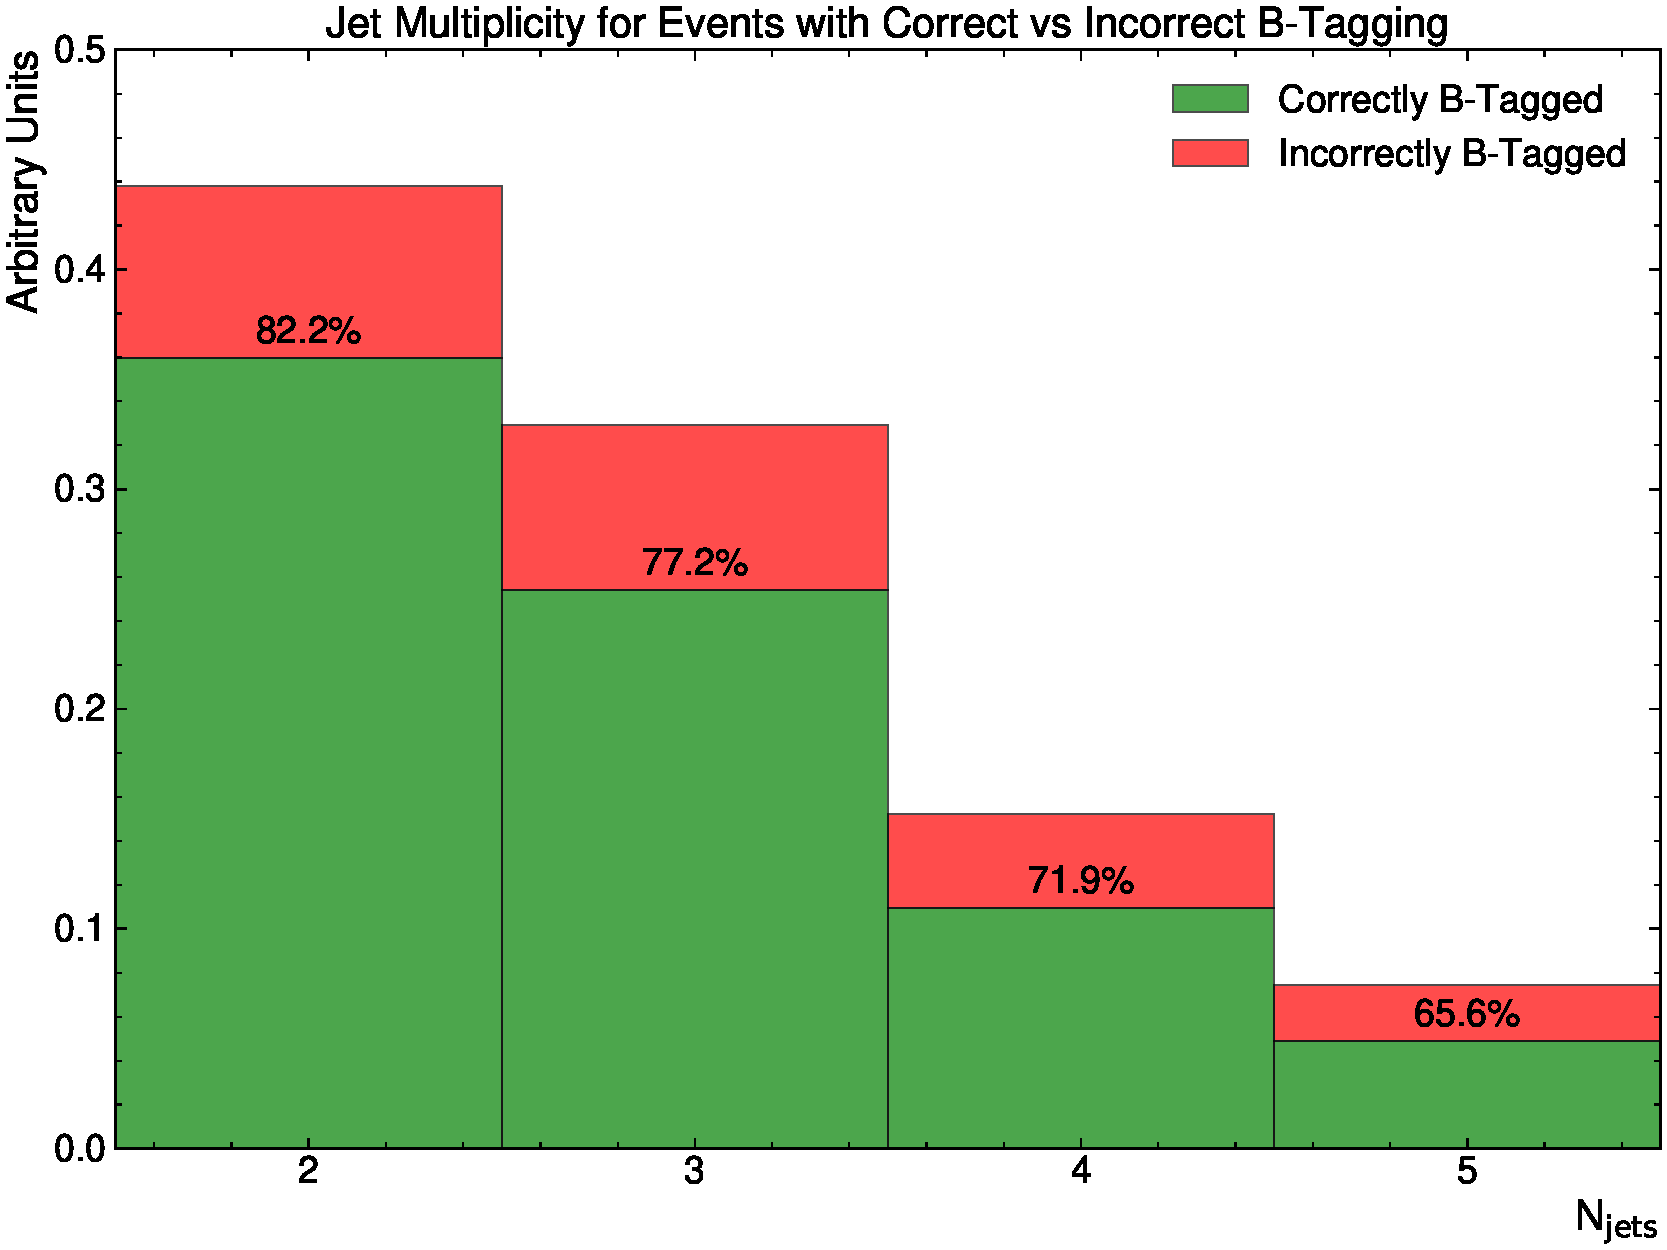
\includegraphics[width=0.7\textwidth]{plots/feature_plots/btagging_performance_by_jet_multiplicity.pdf}
    \caption{This plot shows the b-tagging performance for different numbers of jets in the event. For each jet multiplicity, the number of events, with only jets from top-decays being b-tagged }
\end{figure}

\subsubsection{Threshold Topology}
\label{sec:threshold_topology}
\begin{figure}[H]
    \centering
    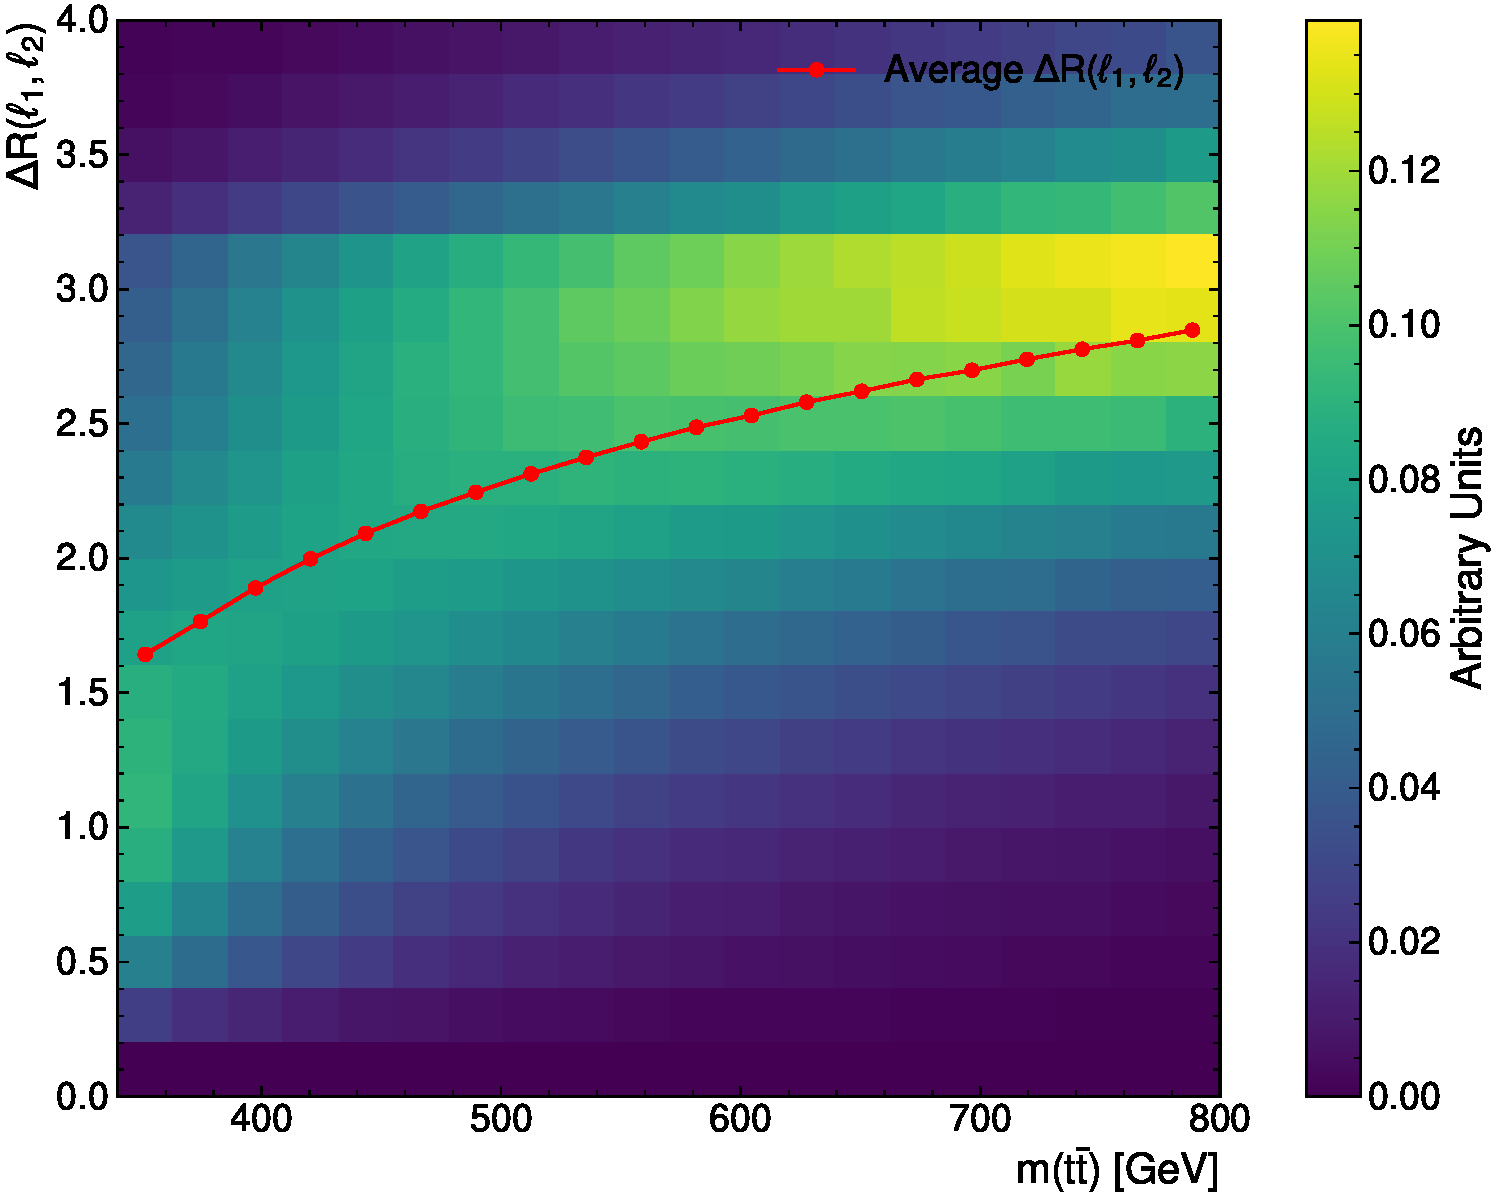
\includegraphics[width=0.7\textwidth]{plots/feature_plots/ttbar_mass_vs_dR_l1l2.pdf}
    \caption{This plot shows the distribution of events binned in the parton-level $m(t\bar{t})$ and the angular distance $\Delta R(\ell_1,\ell_2)$.}
    \label{fig:feature_2d_mttbar_dR_l1l2}
\end{figure}


\begin{figure}[H]
    \begin{subfigure}{0.49\textwidth}
        \centering
        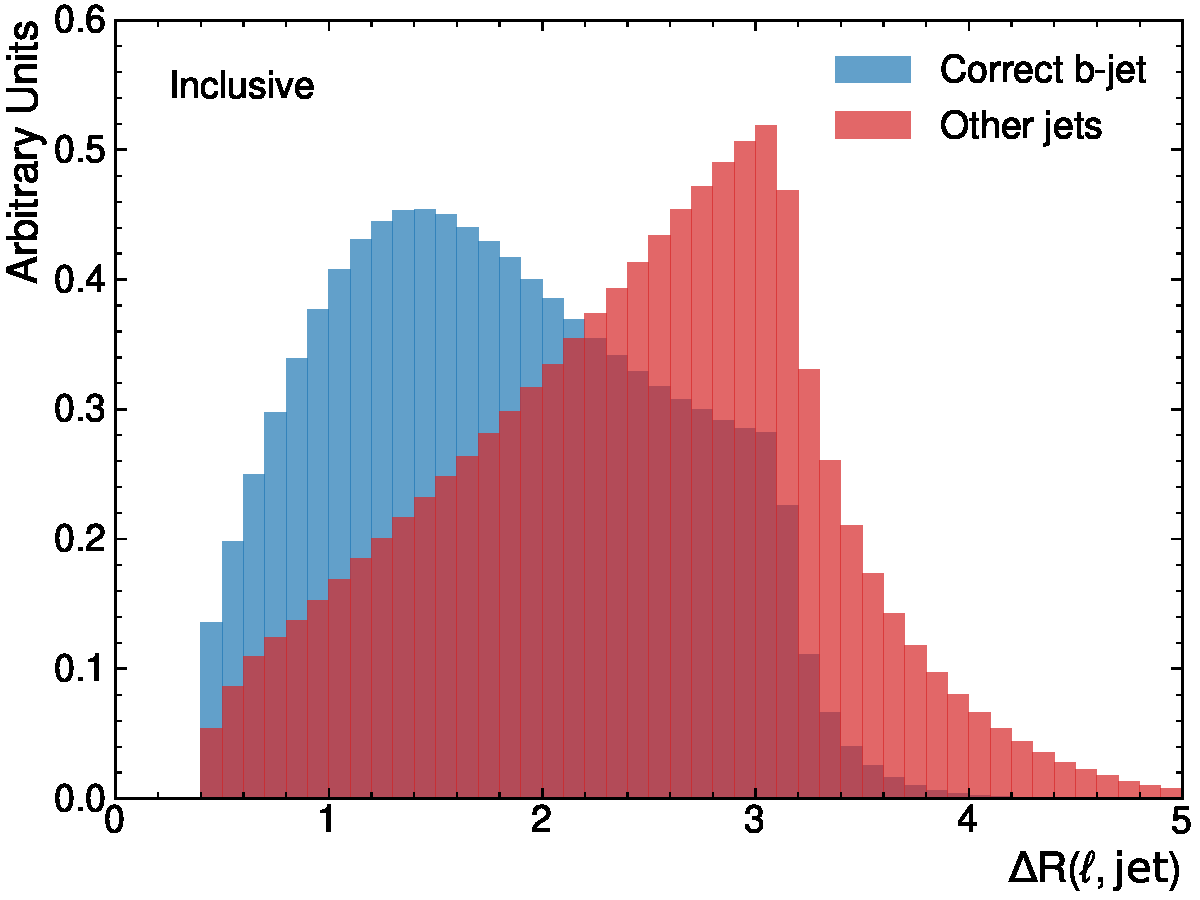
\includegraphics[width=1.0\textwidth]{plots/feature_plots/relational_jet_lepton_deltaR_distribution.pdf}
        \caption{Inclusive}
        \label{fig:deltaR_pairing:inclusive}
    \end{subfigure}
    \begin{subfigure}{0.49\textwidth}
        \centering
        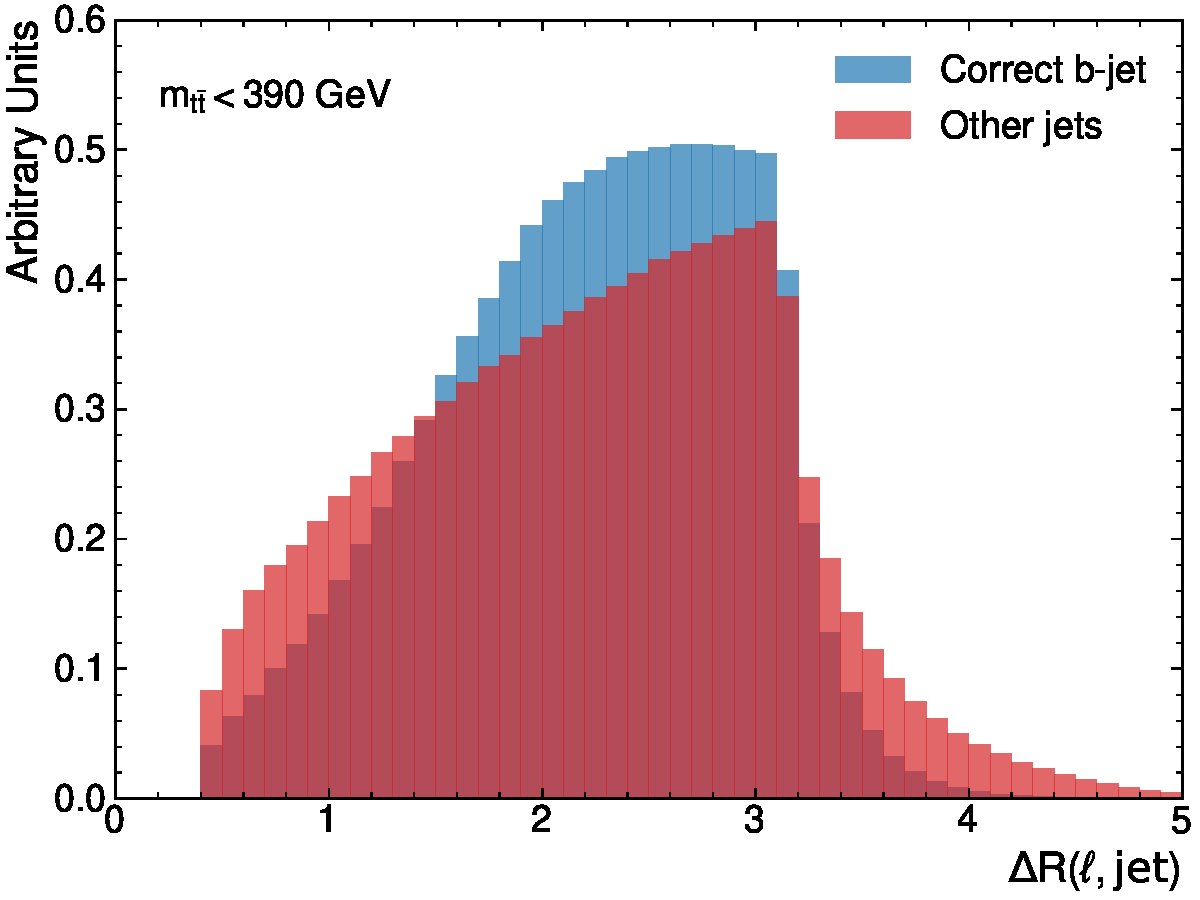
\includegraphics[width=1.0\textwidth]{plots/feature_plots/relational_jet_lepton_deltaR_distribution_m_tt_390GeV.pdf}
        \caption{Near-Threshold}
        \label{fig:deltaR_pairing:threshold}
    \end{subfigure}
    \caption{Distribution of $\Delta R(\ell,j)$ for correct and incorrect pairing of jets and leptons. Evaluated on the full sample in \subrefb{fig:deltaR_pairing:inclusive} and near-threshold in \subrefb{fig:deltaR_pairing:threshold}.}
    \label{fig:deltaR_pairing}
\end{figure}

\begin{figure}[H]
    \begin{subfigure}{0.49\textwidth}
        \centering
        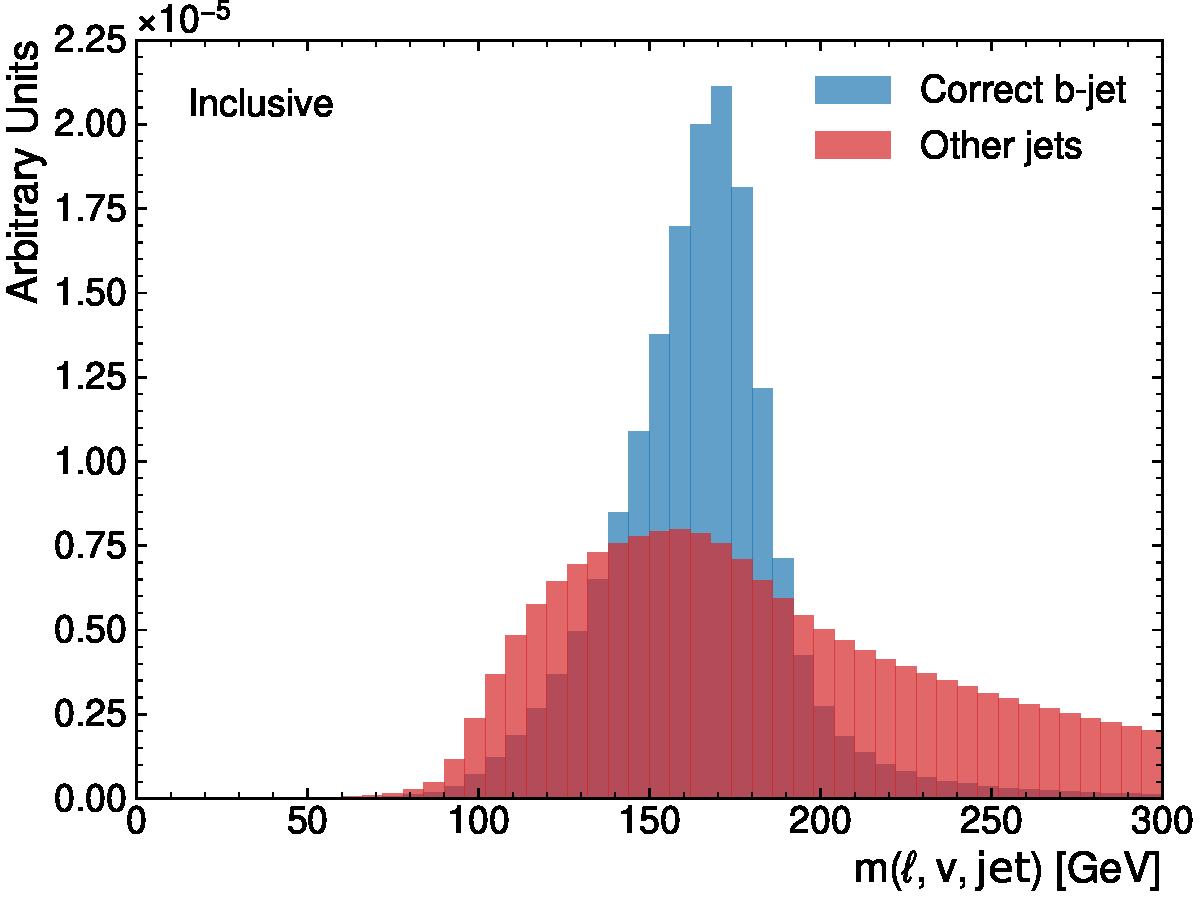
\includegraphics[width=1.0\textwidth]{plots/feature_plots/relational_jet_lepton_full_inv_mass_distribution.pdf}
        \caption{Inclusive}
        \label{fig:invariant_mass_pairing:inclusive}
    \end{subfigure}
    \begin{subfigure}{0.49\textwidth}
        \centering
        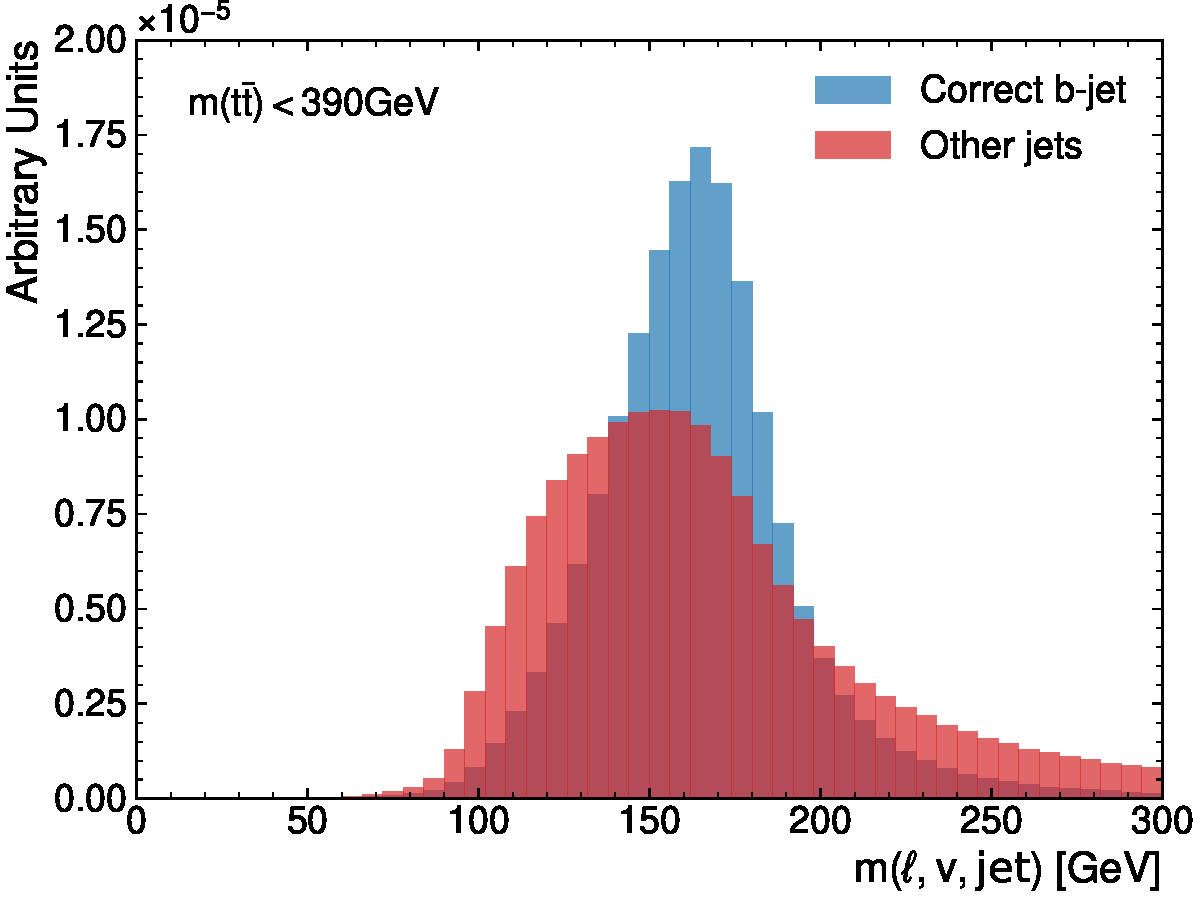
\includegraphics[width=1.0\textwidth]{plots/feature_plots/relational_jet_lepton_full_inv_mass_distribution_m_tt_390GeV.pdf}
        \caption{Near-Threshold}
        \label{fig:invariant_mass_pairing:threshold}
    \end{subfigure}
    \caption{Distribution of $m(\ell,\nu, j)$ for correct and incorrect pairing of jets and leptons. Evaluated on the full sample in \subrefb{fig:invariant_mass_pairing:inclusive} and near-threshold in \subrefb{fig:invariant_mass_pairing:threshold}.}
    \label{fig:invariant_mass_pairing}
\end{figure}



\section{Hyperparameter Optimisation Results}
\label{sec:hyperparams}

\subsection{FeatureConcatTransformer}
\begin{figure}[H]
    \begin{subfigure}{1.0\textwidth}
        \centering
        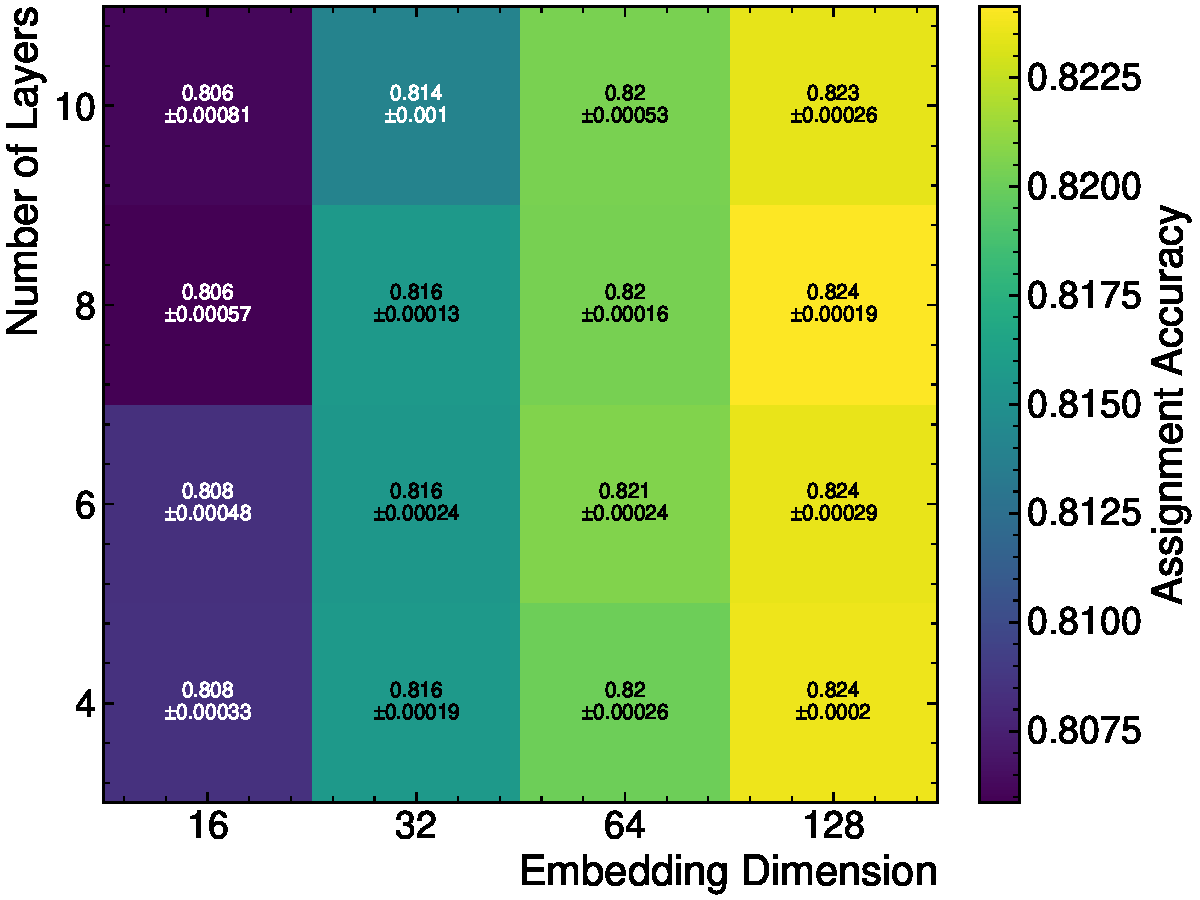
\includegraphics[width=0.7\textwidth]{plots/hyperparams_assignment/FeatureConcatTransformer_assignment_accuracy_embedding_dimension_vs_num_layers.pdf}
        \caption{Assignment Accuracy}
        \label{fig:hyperparams_fct_acc}
    \end{subfigure}
    \begin{subfigure}{1.0\textwidth}
        \centering
        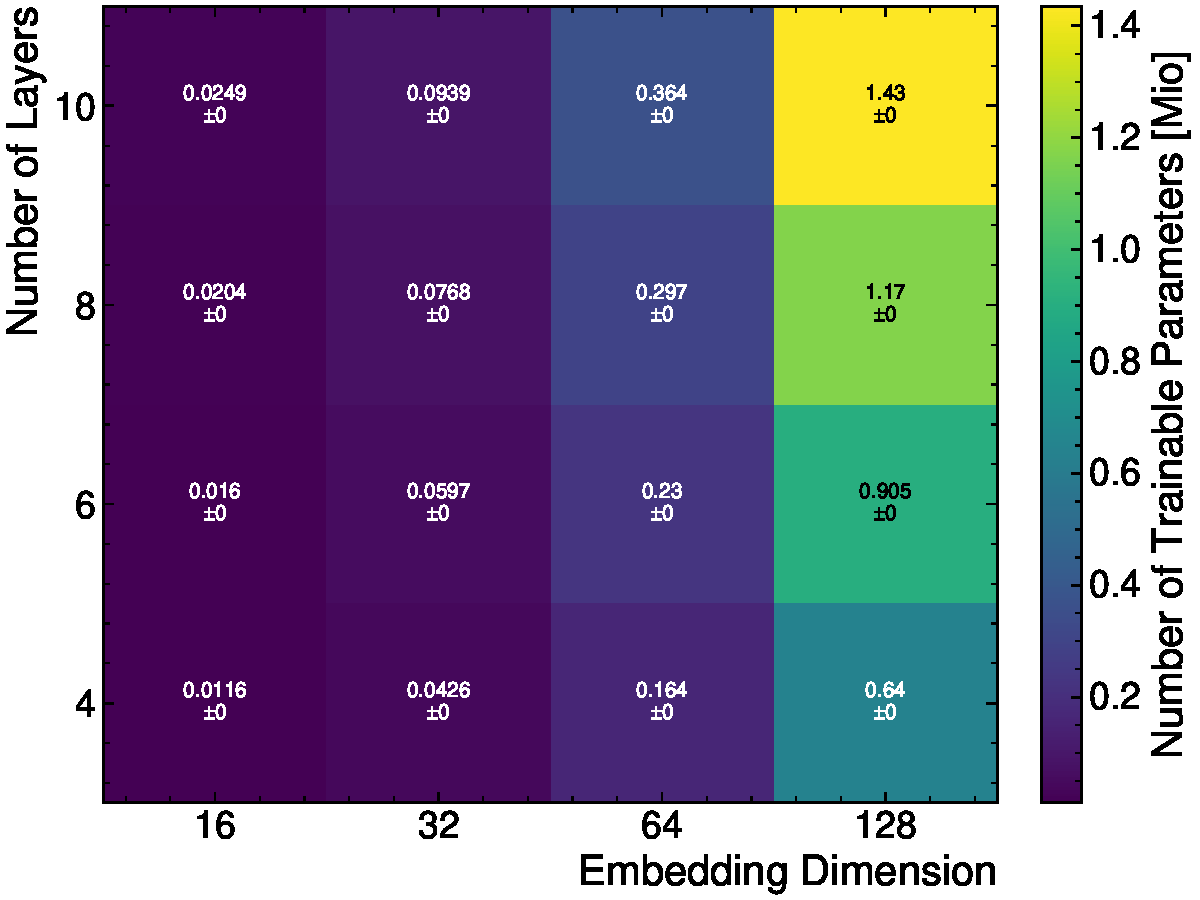
\includegraphics[width=0.7\textwidth]{plots/hyperparams_assignment/FeatureConcatTransformer_num_trainable_parameters_embedding_dimension_vs_num_layers.pdf}
        \caption{Number of Trainable Parameters}
        \label{fig:hyperparams_fct_params}
    \end{subfigure}
    \caption{The Figures \subrefb{fig:hyperparams_fct_acc} and \subrefb{fig:hyperparams_fct_params} show the assignment accuracy and the number of trainable parameters of the FeatureConcatTransformer architecture as a function of the embedding dimension and the number of transformer layers.}
    \label{fig:hyperparams_fct}
\end{figure}

\subsection{CrossAttentionTransformer}
\begin{figure}[H]
    \begin{subfigure}{1.0\textwidth}
        \centering
        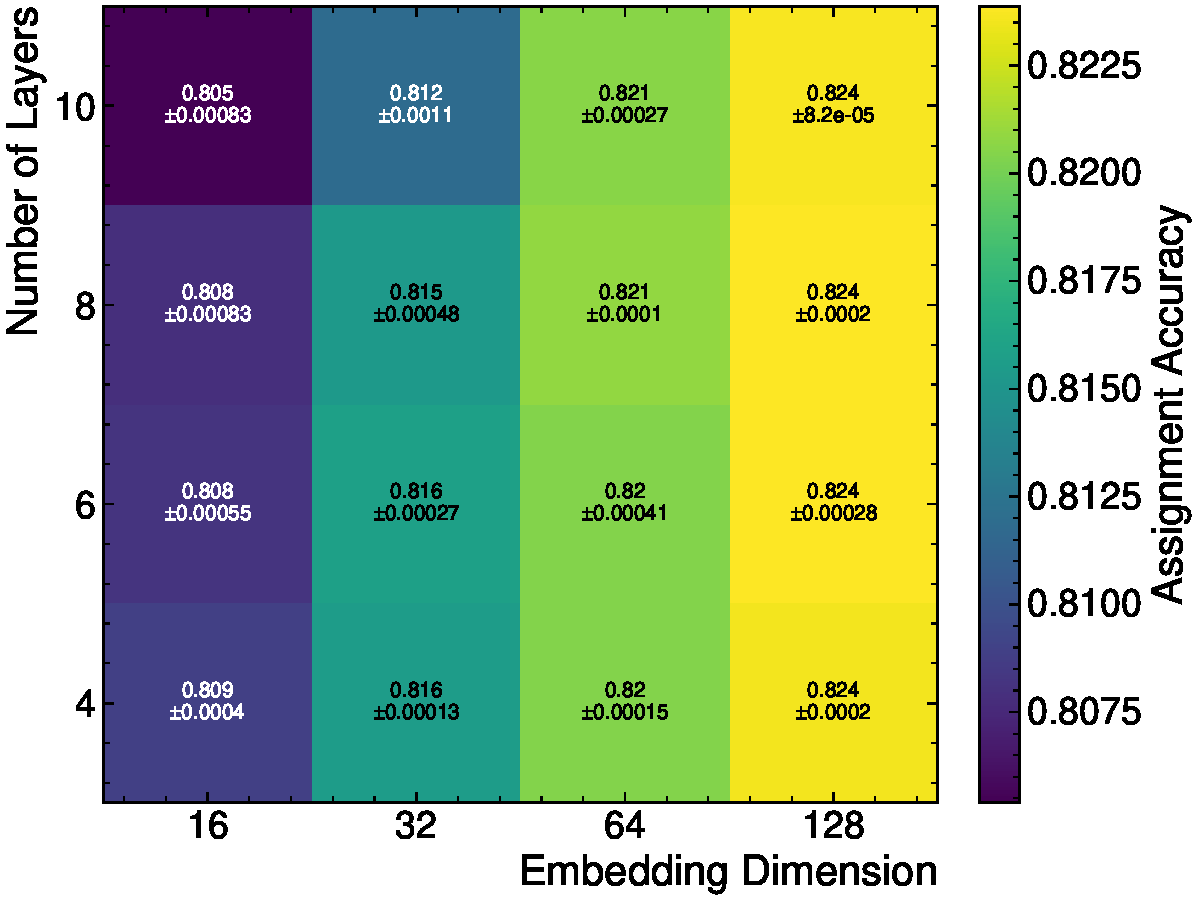
\includegraphics[width=0.7\textwidth]{plots/hyperparams_assignment/CrossAttentionTransformer_assignment_accuracy_embedding_dimension_vs_num_layers.pdf}
        \caption{Assignment Accuracy}
        \label{fig:hyperparams_cat_acc}
    \end{subfigure}
    \begin{subfigure}{1.0\textwidth}
        \centering
        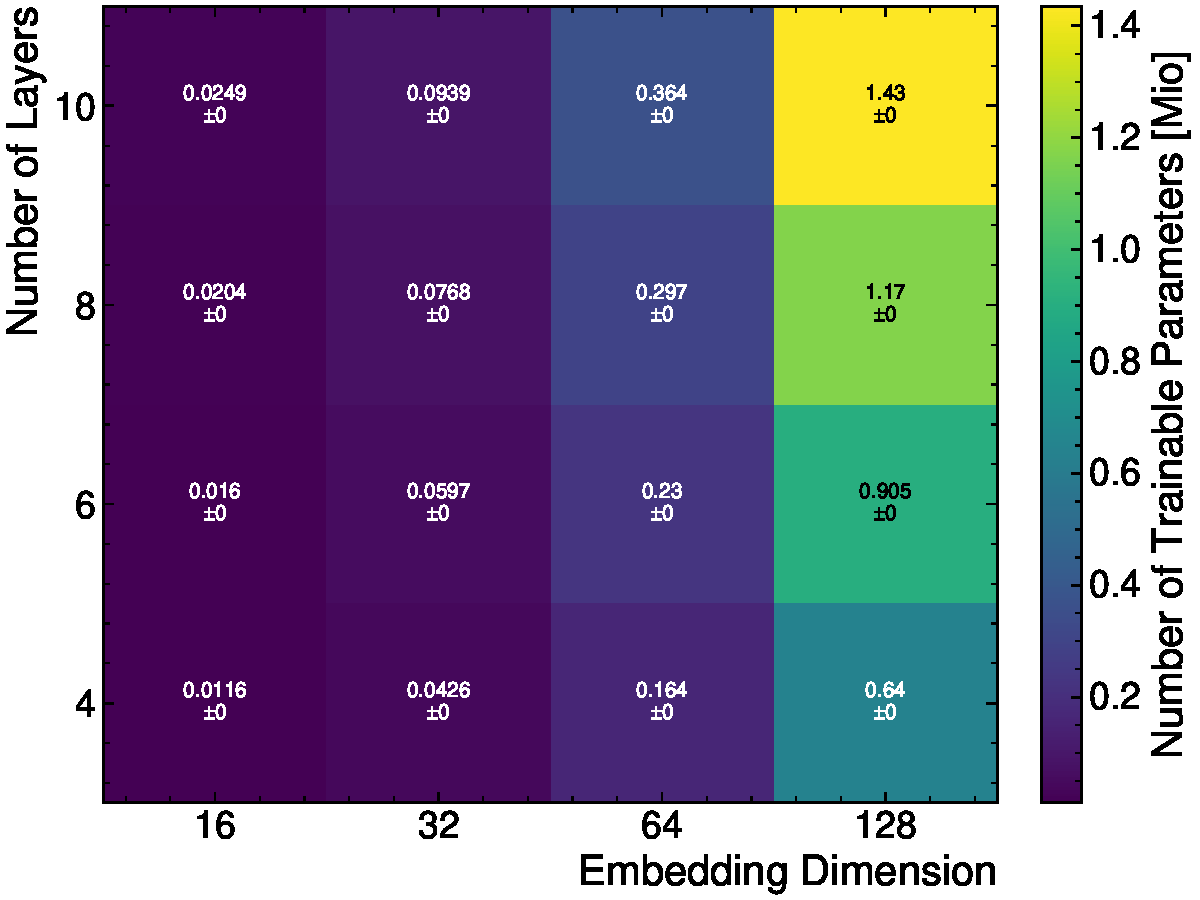
\includegraphics[width=0.7\textwidth]{plots/hyperparams_assignment/CrossAttentionTransformer_num_trainable_parameters_embedding_dimension_vs_num_layers.pdf}
        \caption{Number of Trainable Parameters}
        \label{fig:hyperparams_cat_params}
    \end{subfigure}
    \caption{The Figures \subrefb{fig:hyperparams_cat_acc} and \subrefb{fig:hyperparams_cat_params} show the assignment accuracy and the number of trainable parameters of the CrossAttentionTransformer architecture as a function of the embedding dimension and the number of transformer layers.}
    \label{fig:hyperparams_cat}
\end{figure}

\subsection{CompactTransformer}
\begin{figure}[H]
    \begin{subfigure}{1.0\textwidth}
        \centering
        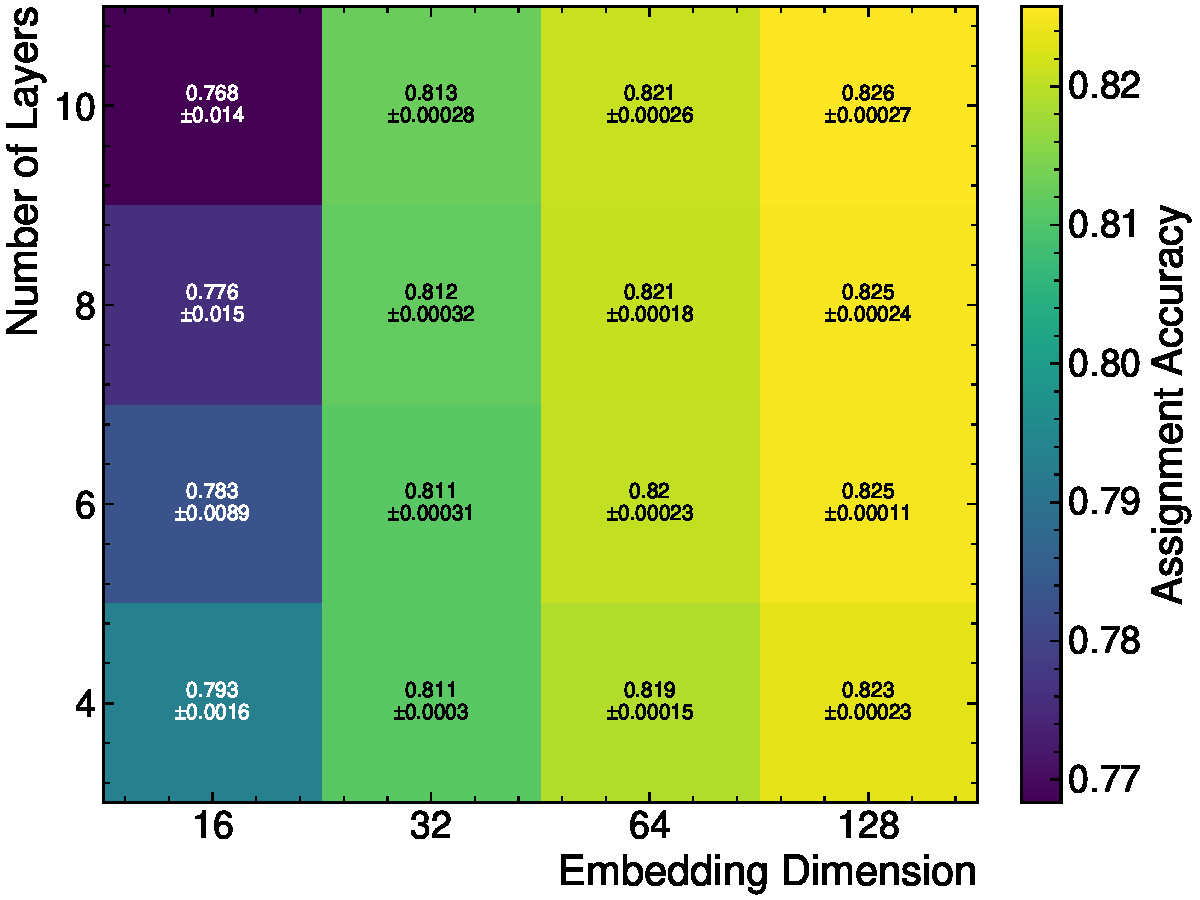
\includegraphics[width=0.7\textwidth]{plots/hyperparams_assignment/CompactTransformer_assignment_accuracy_embedding_dimension_vs_num_layers.pdf}
        \caption{Assignment Accuracy}
        \label{fig:hyperparams_compact_acc}
    \end{subfigure}
    \begin{subfigure}{1.0\textwidth}
        \centering
        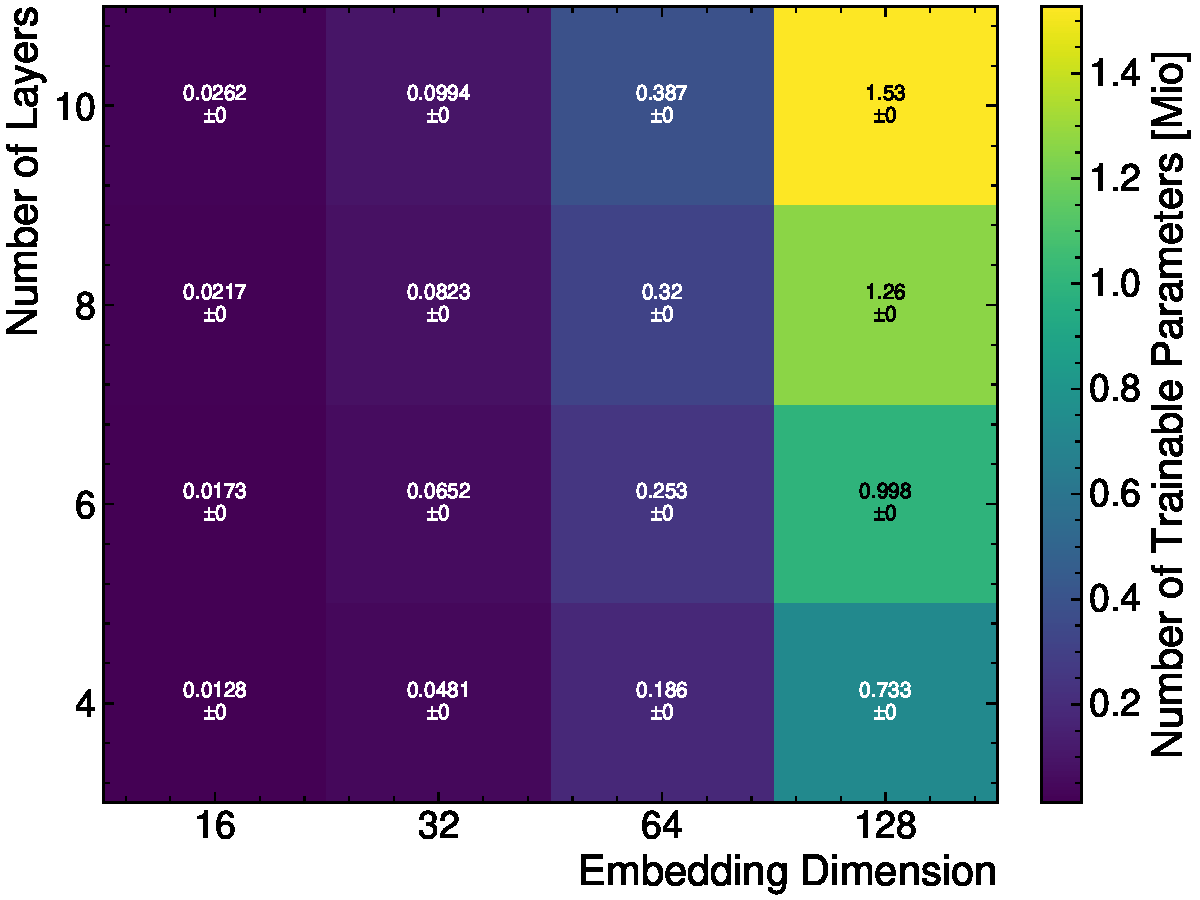
\includegraphics[width=0.7\textwidth]{plots/hyperparams_assignment/CompactTransformer_num_trainable_parameters_embedding_dimension_vs_num_layers.pdf}
        \caption{Number of Trainable Parameters}
        \label{fig:hyperparams_compact_params}
    \end{subfigure}
    \caption{The Figures \subrefb{fig:hyperparams_compact_acc} and \subrefb{fig:hyperparams_compact_params} show the assignment accuracy and the number of trainable parameters of the CompactTransformer architecture as a function of the embedding dimension and the number of transformer layers.}
    \label{fig:hyperparams_compact}
\end{figure}



\section{Performance Plots}
\subsection{Assignment Performance}
\begin{figure}[H]
    \centering
    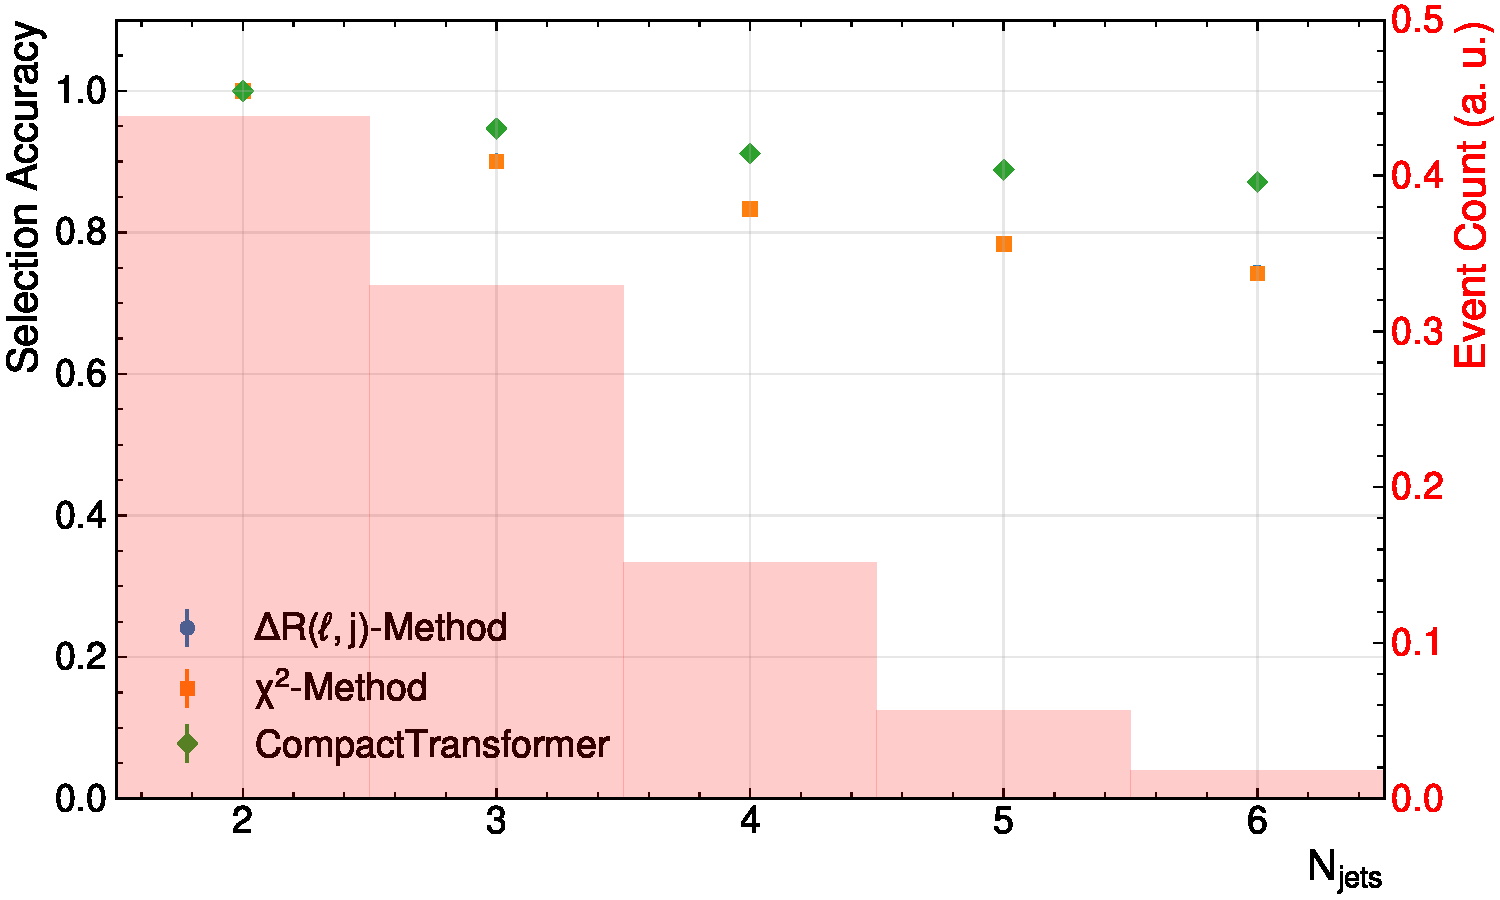
\includegraphics[width=0.7\textwidth]{plots/compact_assigner/binned_performance/N_jets/binned_selection_accuracies_N_jets.pdf}
    \caption{Selection accuracy as a function of the number of jets in the event for different reconstruction methods. The background histograms show of the distribution of events as a function of the number of jets. The uncertainties represent the statistical variations in the evaluation dataset.}
    \label{fig:selection_accuracy_vs_n_jets}
\end{figure}



\begin{figure}
    \centering
    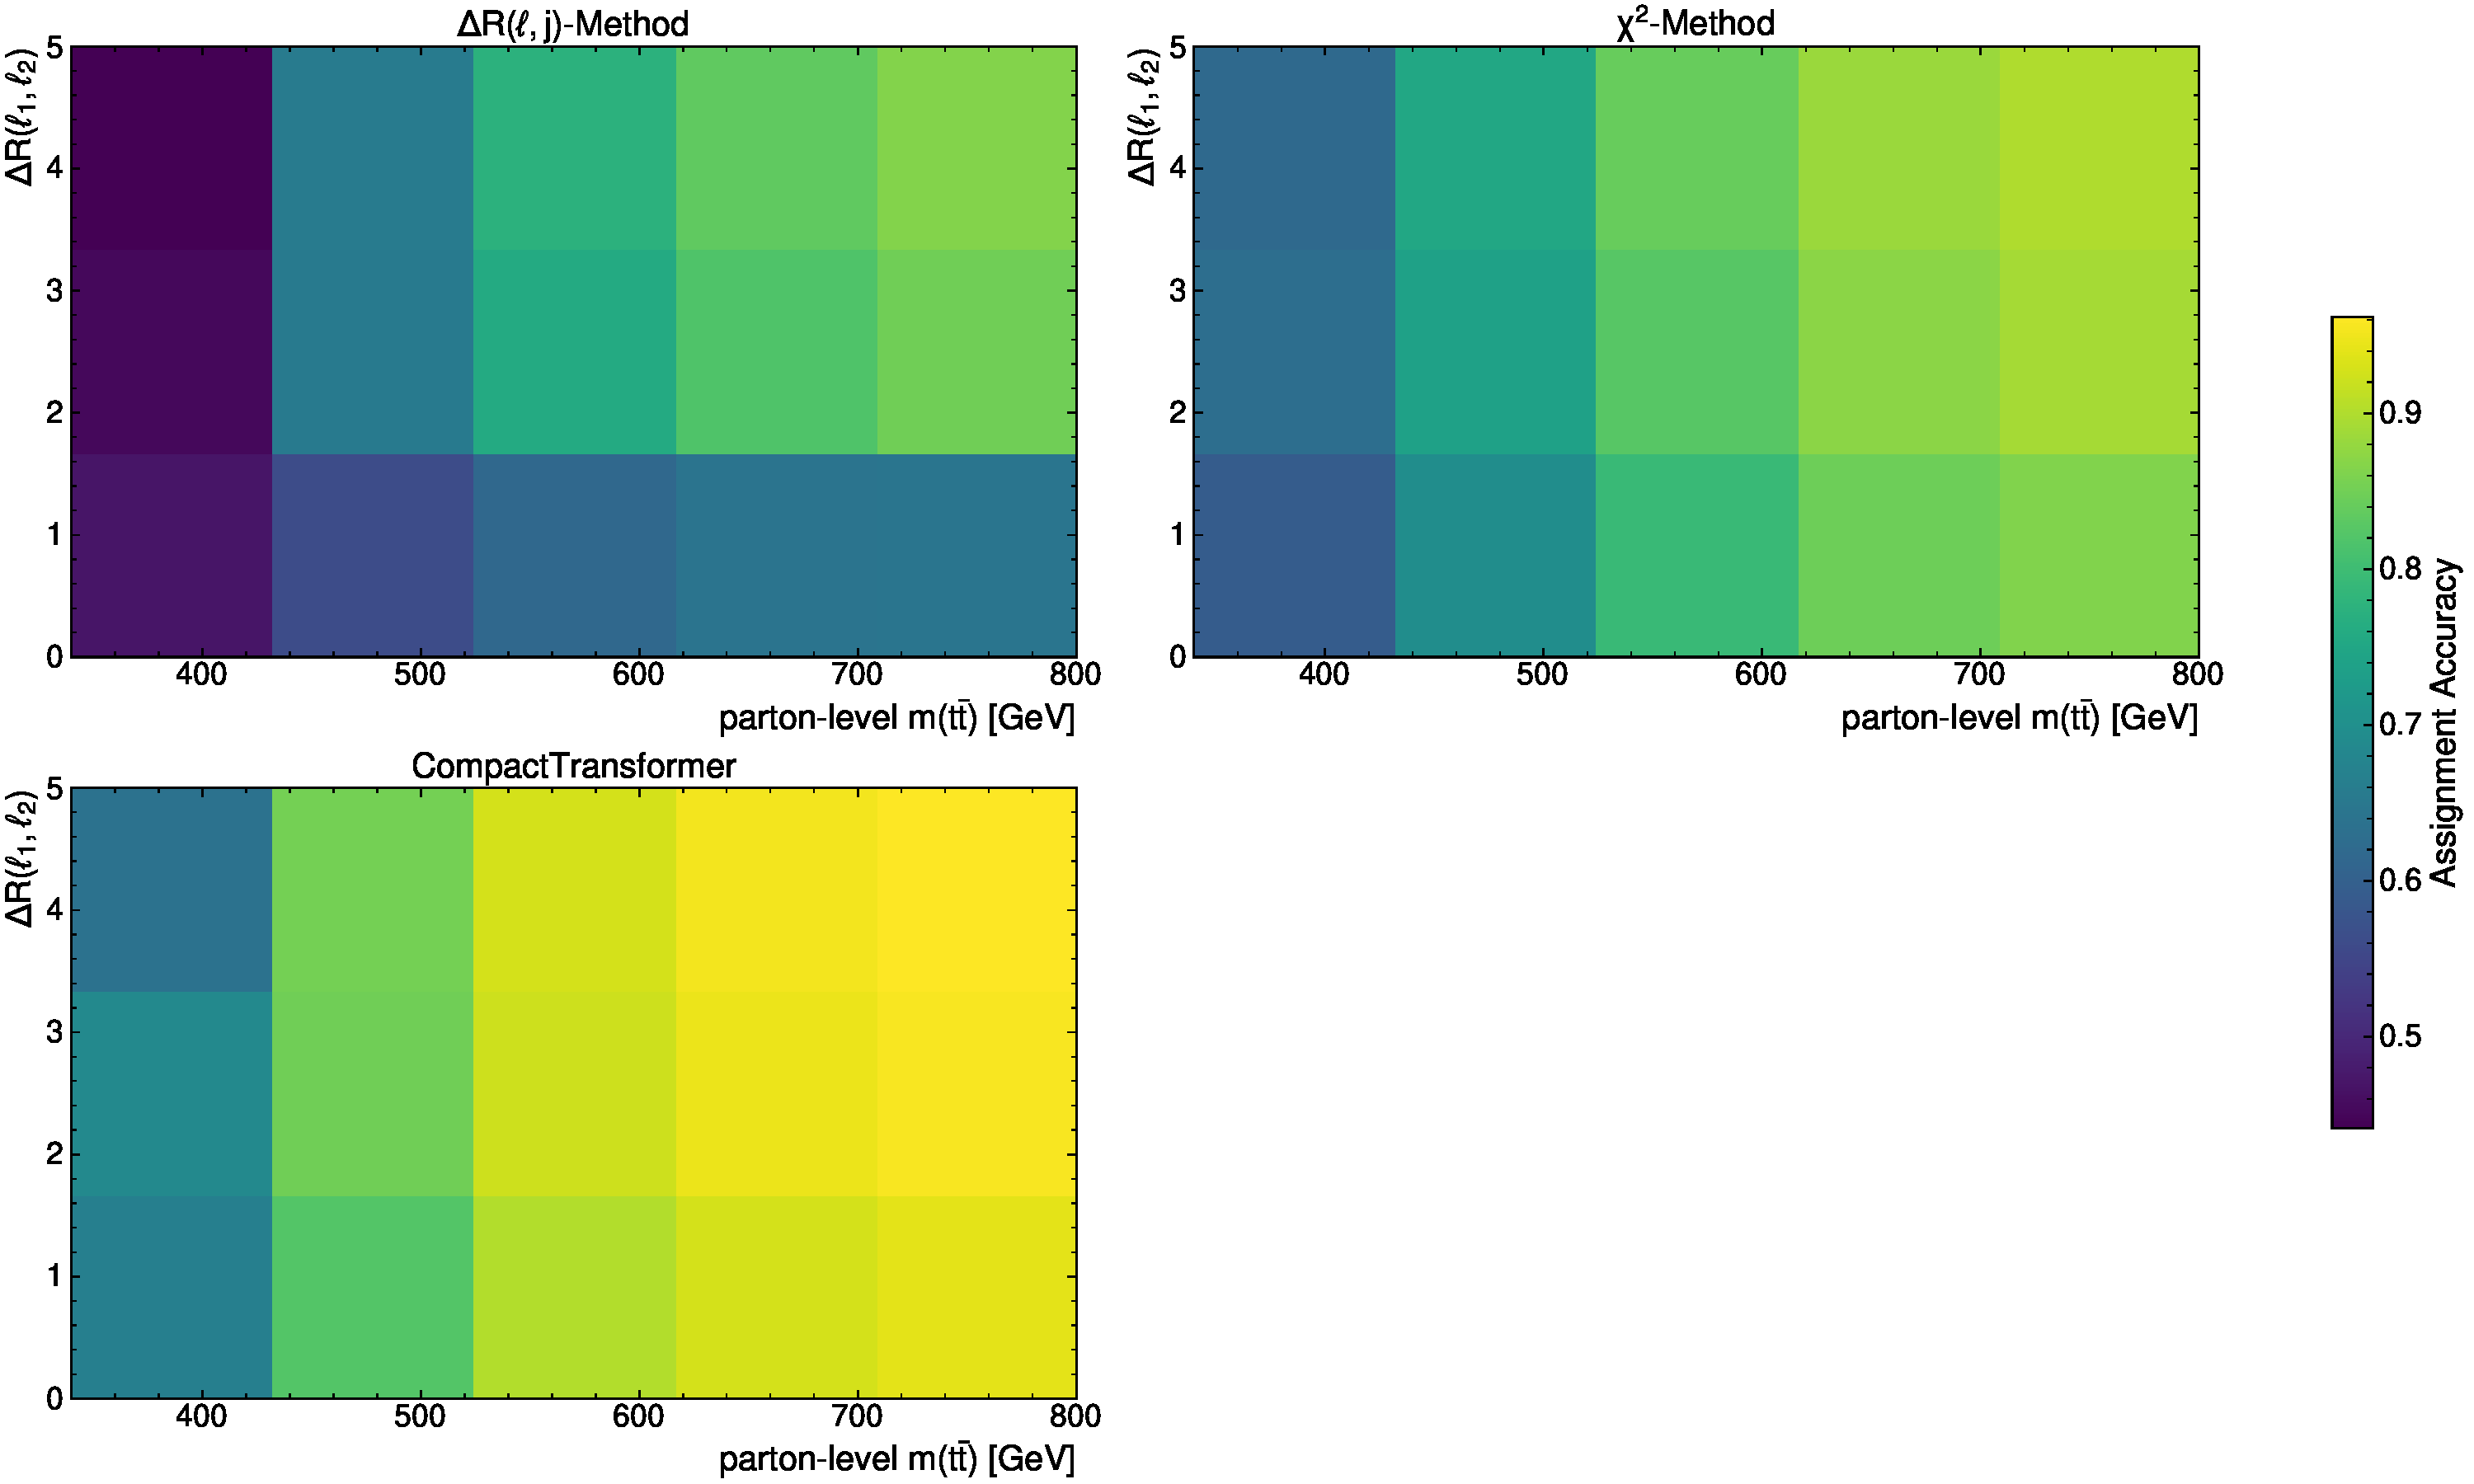
\includegraphics[width=1.0\textwidth]{plots/compact_assigner/binned_2d_performance/truth_ttbar_mass_vs_dR_l1l2/2d_binned_accuracies_truth_ttbar_mass_dR_l1l2.pdf}
    \caption{Assignment accuracy binned with respect to parton-level $m(t\bar{t})$ and $\Delta R(\ell_1,\ell_2)$.}
    \label{fig:accuracy_2d_mttbar_dR_l1l2}
\end{figure}